\documentclass[conference]{IEEEtran}
\IEEEoverridecommandlockouts
% The preceding line is only needed to identify funding in the first footnote. If that is unneeded, please comment it out.
\usepackage[T1]{fontenc}
\usepackage[utf8]{inputenc}
\usepackage{cite}
\usepackage{amsmath,amssymb,amsfonts}
\usepackage{algorithmic}
\usepackage{algorithm}
\usepackage{float}
\usepackage{placeins}
\usepackage{graphicx}
\usepackage{textcomp}
\usepackage{xcolor}
\usepackage{booktabs}
\usepackage{array}
\usepackage{tabularx}
\usepackage{longtable}
\usepackage{multirow}
\usepackage{caption}
\captionsetup[table]{labelfont={sc,small},textfont={sc,small},justification=centering,labelsep=newline,skip=10pt}
\captionsetup[algorithm]{labelfont={bf},font={small},justification=raggedright,singlelinecheck=false}
\captionsetup[figure]{labelfont={bf},justification=centering,skip=10pt}

\def\BibTeX{{\rm B\kern-.05em{\sc i\kern-.025em b}\kern-.08em
    T\kern-.1667em\lower.7ex\hbox{E}\kern-.125emX}}
\begin{document}

\title{[CSE299(1) - Group\#6] Final Report: Home Healthcare \& Diagnostic Center Management System\\
{\large Summer 2026}
}

\author{
\IEEEauthorblockN{
    Md Mehrab Hossain Khandoker (2311511042),\\
    Nafsin Nasama Salmee (2311776642),\\
    Mohammed Mushfiq Syed (2232295042),\\
    Yousuf Jamil (2321210642)
}
\IEEEauthorblockA{\textit{Department of Electrical and Computer Engineering}\\
\textit{North South University}\\
Dhaka, Bangladesh \\
\{mehrab.khandoker, nafsin.salmee, mohammed.syed, yousuf.jamil.232\}@nothsouth.edu}
}

\maketitle

\begin{abstract}
The Home Healthcare \& Diagnostic Center Management System (HHDMS) is a centralized, multi-role digital platform integrating call-center dispatch, electronic medical record (EMR) management, telemedicine, field-logistics tracking, mobile point-of-care diagnostics, and automated billing into a single cross-platform ecosystem. HHDMS is developed as a distributed system comprising a NestJS~11 REST and Socket.IO backend, a Next.js~16 administrative web application, and a Jetpack Compose Android client, backed by a Prisma ORM and PostgreSQL (Neon) database. The platform supports more than ten operational roles---including call-center agents, MBBS doctors, specialists, nurses, caregivers, nutritionists, sonologists, X-ray technicians, administrators, and patients---under a unified Role-Based Access Control (RBAC) framework. Key subsystems include an interactive DICOM imaging suite, WebRTC video consultations, real-time messaging, Stripe payment processing, GPS-verified field operations, and a standalone Android nurse application. The system achieved near-total coverage of the course Software Requirements Specification (SRS) and reached staging deployment readiness. The document details the architecture, module implementations, security measures, and individual contributions.
\end{abstract}

\begin{IEEEkeywords}
Home healthcare, telemedicine, electronic medical records, DICOM imaging, GPS tracking, role-based access control, real-time communication, mobile health
\end{IEEEkeywords}

\section{Introduction}

\subsection{Project Overview}
Access to timely, efficient, and comprehensive healthcare remains a critical challenge globally, particularly in developing and densely populated regions~. Traditional healthcare delivery relies heavily on physical hospital visits, which often result in prolonged waiting times, increased financial burden, heightened risk of nosocomial infections, and severe logistical challenges for vulnerable demographics---including elderly, chronically ill, pediatric, and post-surgical patients~.

To address these systemic inefficiencies, the \textbf{Home Healthcare \& Diagnostic Center Management System (HHDMS)} introduces a centralized, multi-role digital ecosystem designed to bridge the gap between primary clinical care, specialized medical services, field nursing, home caregiving, and mobile diagnostic operations~\cite{srs2026}. By combining call-center dispatching, real-time field logistics, EMR management, dynamic scheduling, mobile point-of-care diagnostics, and telehealth capabilities into a unified architecture, HHDMS transforms home healthcare from a fragmented service model into an integrated, end-to-end clinical workflow~\cite{srs2026}.

This report documents the complete design and implementation of HHDMS, from requirements through architectural decisions to the operationalized modules and their evaluation against the course Software Requirements Specification (SRS)~\cite{srs2026}.

\subsection{Problem Statement}
Despite the growing demand for decentralized and home-based medical services, existing healthcare systems suffer from severe operational limitations~:
\begin{itemize}
\item \textbf{Fragmented Operational Silos:} Patient intakes, teleconsultations, home nursing visits, and diagnostic testing operate as disconnected services, leading to lost records and poor care continuity~\cite{srs2026}.
\item \textbf{Inadequate Dispatch and Field Visibility:} Traditional management relies on manual scheduling without real-time tracking, so operators lack visibility into provider locations, dynamic ETA predictions, or geofenced visit attendance~\cite{zandbergen2009accuracy}.
\item \textbf{Inaccessible Point-of-Care Diagnostics:} Mobile diagnostic imaging at the bedside remains technically isolated; without native DICOM support, specialists cannot remotely review, measure, and annotate scans in real time~\cite{pacs2001, dicom2021}.
\item \textbf{Heterogeneous Workflows and Security Gaps:} Managing diverse clinical and non-clinical professionals under a unified, role-aware security framework presents a complex challenge~.
\end{itemize}

\subsection{Objectives}
The primary objective of HHDMS is to design, develop, and deploy a robust, scalable, multi-tenant digital healthcare management system~\cite{srs2026}. Specific goals include:
\begin{enumerate}
\item \textbf{Centralized Lifecycle Management:} A streamlined intake pipeline via call-center ticket dispatch, structured referral chains, and unified Medical Record Numbers (MRNs) preserving complete patient history~\cite{srs2026}.
\item \textbf{Real-Time Field Optimization:} Automated resource allocation, GPS tracking, route estimation, and dynamic geofenced check-in/out verification for field personnel~\cite{zandbergen2009accuracy}.
\item \textbf{Advanced Point-of-Care Diagnostics:} Bedside DICOM imaging capture for ultrasound and X-ray services backed by an interactive web viewer for remote specialist analysis~\cite{dicom2021, pacs2001}.
\item \textbf{Integrated Telehealth and Communication:} Secure, low-latency video/audio teleconsultations, instant messaging, and automated notifications across mobile and web platforms~\cite{fette2011websocket, agorawebrtc}.
\end{enumerate}

\subsection{Scope of the System}
HHDMS encompasses a cross-platform solution comprising a high-performance backend REST API and WebSocket engine, an administrative web application, and a feature-rich mobile client~\cite{srs2026}. The platform supports more than ten distinct operational roles, including call-center agents, general practitioners (MBBS), specialist doctors, nurses, caregivers, nutritionists, sonologists, X-ray technicians, system administrators, and patients~\cite{srs2026}. Through this framework, HHDMS governs every phase of home healthcare---from primary contact and dynamic triage to treatment planning, point-of-care diagnostic delivery, and automated billing~\cite{srs2026}.

\section{Background and Related Work}

\subsection{Domain Context}
Over recent years, the global healthcare ecosystem has shifted from centralized hospital visits toward decentralized, patient-centric care delivery~. Home healthcare and telehealth have emerged as critical infrastructures to alleviate hospital congestion, reduce costs, and provide continuous care, particularly in regions such as Bangladesh where urban traffic and overburdened facilities present significant barriers to timely intervention~\cite{srs2026}. A modern home healthcare infrastructure requires more than basic teleconsultations; it demands a unified platform capable of orchestrating multi-disciplinary operations across 11 clinical specialties, adult and pediatric nursing, specialized caregiving, and mobile diagnostics~\cite{srs2026}.

\begin{itemize}
\item \textbf{Chronic-care and elderly populations} benefit most from home-delivered clinical and non-clinical services, reducing travel burden and exposure to hospital-acquired infections~.
\item \textbf{Field logistics} (nurse and caregiver dispatch) require real-time location awareness and verifiable attendance to ensure safety and accountability~\cite{zandbergen2009accuracy}.
\item \textbf{Point-of-care imaging} (ultrasound and portable X-ray) needs standards-based DICOM support to enable remote specialist interpretation away from fixed facilities~\cite{dicom2021, pacs2001}.
\end{itemize}

\subsection{Comparative Analysis}
Existing digital healthcare platforms fall into three categories, each with architectural limitations for comprehensive home healthcare. Table~\ref{tab:related} summarizes the comparison.

\begin{table}[htbp]
\centering
\small
\setlength{\tabcolsep}{3pt}
\renewcommand{\arraystretch}{1.2}
\begin{tabularx}{\columnwidth}{>{\raggedright\arraybackslash}p{0.30\columnwidth} >{\raggedright\arraybackslash}p{0.28\columnwidth} >{\raggedright\arraybackslash}X}
\toprule
\textbf{System Category} & \textbf{Core Functionality} & \textbf{Operational Gaps in Home Care} \\
\midrule
\textbf{Standard Telemedicine Apps} & Video/audio consultations, e-prescriptions, basic scheduling & No field dispatch, GPS tracking, home nursing, or portable diagnostic workflows~ \\
\textbf{Hospital Information Systems (HIS/EMR)} & In-hospital bed management, billing, laboratory management & Fixed-location only; no field geofencing, map tracking, offline capability, or call-center dispatch~\cite{pacs2001} \\
\textbf{Standalone Dispatch / Logistics} & Field-worker tracking, booking, proof of arrival & No clinical capability: ICD-10 coding, drug-interaction checking, DICOM viewers, multi-specialty workflows~\cite{who2016icd10, dicom2021} \\
\bottomrule
\end{tabularx}
\caption{Comparative analysis of digital healthcare system categories.}
\label{tab:related}
\end{table}

HHDMS bridges these gaps by combining clinical governance, diagnostic capability, and field logistics into a single centralized platform~\cite{srs2026}.

\section{System Architecture}

HHDMS is architected as a distributed, multi-tier ecosystem comprising three principal layers~\cite{fette2011websocket}:

\begin{itemize}
\item \textbf{Backend API Layer:} A NestJS~11 REST API with Socket.IO WebSocket gateways~, Prisma ORM over PostgreSQL (Neon), Passport JWT authentication~\cite{jones2015jwt}, Firebase Admin SDK, Stripe SDK~\cite{stripe2024api}, and Agora token generation~\cite{agorawebrtc}. This layer exposes modular controllers and services for each clinical desk and is the single source of truth for clinical data.
\item \textbf{Administrative Web Layer:} A Next.js~16 App Router application~ with Tailwind CSS, a Socket.IO client for real-time updates, Cornerstone.js for DICOM rendering~\cite{dicom2021}, and PDF/annotation tooling. This layer serves call-center agents, MBBS doctors, specialists, sonologists, nutritionists, X-ray technicians, and administrators.
\item \textbf{Mobile Client Layer:} A Jetpack Compose Android application providing patient, field-doctor, caregiver, and nurse experiences, using Retrofit, Socket.IO, Agora RTC, osmdroid/OSRM for mapping~\cite{osmdroid2024}, Stripe PaymentSheet, and Firebase Cloud Messaging~\cite{firebase2024fcm}.
\end{itemize}

All subsystems are governed by a unified Role-Based Access Control (RBAC) mechanism~, built as a Turborepo monorepo (npm workspaces) for the web/backend and a Gradle multi-module project for the Android clients.

\subsection{Real-Time Communication Subsystem}
Real-time requirements are satisfied through multiple Socket.IO namespaces~\cite{fette2011websocket}. Each clinical interaction domain (visits, chat, video-call signaling, dashboard rooms) is isolated into its own gateway, routing users into private rooms so that state updates---appointment badges, chat messages, typing indicators, and incoming-call notifications---are delivered without full-page refreshes. A dedicated \texttt{allowEIO3} compatibility flag enables interoperability with the legacy Android Socket.IO~v2 client.

\subsection{Security Architecture}
Security is enforced through layered safeguards~\cite{jones2015jwt}:
\begin{itemize}
\item \textbf{Authentication:} Passport-based JWT strategy~\cite{jones2015jwt} validates every client request; tokens encode the user's role and identity.
\item \textbf{Authorization:} A fine-grained \texttt{RolesGuard} RBAC matrix is applied across all PII and diagnostic endpoints via custom NestJS decorators, ensuring zero-leakage data isolation between roles.
\item \textbf{Middleware guards:} Validation middleware (e.g., \texttt{ensurePatientArrived()}) blocks unauthorized access to sensitive clinical dashboards~\cite{androutsellis2004middleware}.
\item \textbf{Audit logging:} An \texttt{audit\_logs} model records operational access history for compliance.
\end{itemize}

\section{System Modules}

The platform implements the full home healthcare lifecycle through the modules described below. Each module follows the same architectural pattern: a NestJS service and controller exposing REST endpoints, a Prisma data model, and dedicated web and/or Android interfaces for the relevant role.

\subsection{Call-Center Dispatch}
The call-center module provides an agent desktop with inbound caller identification, a live stateful ticket queue with wait-time estimation, and automated ticket generation (\texttt{TKT-YYYY-XXXXX}). An emergency triage protocol auto-flags high-severity requests based on symptom keywords and alerts on-duty MBBS doctors via push notifications, enabling one-click call bridging and escalation~\cite{srs2026}. Agents can log patient requests and allocate available doctors through a unified operational interface.

\subsection{MBBS Primary Care}
The MBBS module supports the full primary-care consultation workflow~\cite{srs2026}: patient vitals recording (BP, pulse, temperature, SpO2, respiratory rate, weight, height), ICD-10 diagnosis management with searchable symptom logging~\cite{who2016icd10}, prescription creation with conditional and taper medications, diagnostic test ordering, emergency flag management, specialist referral creation, digital signature handling, and downloadable PDF prescriptions. Real-time visit synchronization between the doctor and patient applications is handled by a Socket.IO gateway.

\subsection{Specialist Consultation and Medical Imaging}
The specialist module provides a full consultation workspace integrating referral management, dynamic schema-driven diagnosis forms across 11 medical specialties (backed by 16 pre-seeded clinical evaluation protocols), a rule-based drug-interaction checker covering 120+ medication pairs with severity classification, and DICOM imaging~\cite{dicom2021}. An interactive Cornerstone.js-based viewer supports windowing, zoom, pan, multi-frame navigation, and an HTML5 Canvas overlay for vector annotations (freehand, rectangles, labeled arrows, text, measurement) with undo/redo~\cite{pacs2001}. The annotation pipeline transforms screen-space vectors into invariant DICOM pixel-space coordinates prior to rendering.
\begin{figure}[!htb]
\centering
\includegraphics[width=\columnwidth]{dicom_viewer.png}
\caption{Interactive DICOM viewer with windowing, zoom, pan, and Canvas-based vector annotations in the specialist diagnostic workspace.}
\label{fig:dicom_viewer}
\end{figure}

\subsection{Telehealth: Video Consultation and Chat}
A peer-to-peer WebRTC video-consultation subsystem is built on the Agora RTC SDK~\cite{agorawebrtc} and coordinated through a custom Socket.IO signaling gateway handling ringing state transitions, room allocation, and UID-based token generation, integrated on both web and Android. A real-time chat system provides appointment-scoped rooms, message persistence, typing indicators, and read receipts~\cite{fette2011websocket}, with UI components on the web dashboard and the Android patient application. Algorithm~\ref{alg:tele} describes the end-to-end teleconsultation session, from specialist-initiated ringing through Agora channel join to session termination and cleanup. Figure~\ref{fig:teleconsultation} shows the active video-consultation session with ringing state, participant controls, and the Agora media stream.
\begin{figure}[!htb]
\centering
\includegraphics[width=\columnwidth]{teleconsultation.png}
\caption{Active WebRTC teleconsultation session showing the patient and doctor streams with session and call controls.}
\label{fig:teleconsultation}
\end{figure}

\begin{algorithm}[htbp]
\caption{Teleconsultation session management.}
\label{alg:tele}
\begin{algorithmic}[1]
\STATE \textbf{Input:} specialist $S$, patient $P$, consultation room $R$
\STATE $S$ initiates video call to $P$ via Socket.IO signaling gateway
\STATE gateway emits \texttt{video-call:ringing} to $P$'s room
\IF{$P$ accepts the call}
  \STATE gateway generates Agora RTC token for $R$ \COMMENT{UID: specialist=1, patient=2}
  \STATE both clients join channel $R$ with their UID
  \STATE conduct live audio/video session via Agora RTC SDK
  \STATE on consent, gateway logs consultation metadata and starts timer
\ELSE
  \STATE $P$ declines or call times out after 30~seconds
  \STATE gateway notifies $S$ and cancels the session
\ENDIF
\STATE \textbf{Terminate:} either party ends the call
\STATE gateway triggers \texttt{video-call:end} and releases Agora resources
\STATE \textbf{Output:} completed teleconsultation with both participants disconnected cleanly
\end{algorithmic}
\end{algorithm}

\FloatBarrier

\subsection{Caregiver and Field Operations}
The caregiver module supports assigned-patient management, activity logging, and condition-report submission with targeted alerts to supervising clinical staff. GPS-verified check-in/out utilizes \texttt{FusedLocationProviderClient} capture validated against registered patient locations using Haversine distance calculations~, with automatic timesheet generation from check-in/out records~\cite{zandbergen2009accuracy}. Algorithm~\ref{alg:geofence} validates the reported location against the registered patient coordinates before authorizing a shift check-in, mitigating location spoofing.

\begin{algorithm}[htbp]
\caption{GPS-verified caregiver check-in validation.}
\label{alg:geofence}
\begin{algorithmic}[1]
\STATE \textbf{Input:} reported GPS $(\phi_r,\lambda_r)$, registered patient GPS $(\phi_p,\lambda_p)$, geofence radius $d_{\max}$ in meters
\STATE compute Haversine distance $d \leftarrow \text{Haversine}(\phi_r,\lambda_r,\phi_p,\lambda_p)$
\IF{$d \le d_{\max}$}
  \STATE authorize check-in and record $(\phi_r,\lambda_r)$ with timestamp
  \STATE start shift time tracking
\ELSE
  \STATE reject check-in with location-mismatch error
\ENDIF
\STATE \textbf{Output:} authorized or rejected check-in
\end{algorithmic}
\end{algorithm}

\subsection{Nutritionist Workbench}
The nutritionist module provides anthropometric record management with BMI and waist-to-hip ratio calculations and BMI category classification, a localized meal-slot diet planner, calorie and macro calculations, adherence scoring, follow-up scheduling, and a food-item catalog with per-100g nutritional data~\cite{srs2026}. A type-safe analytical service (\texttt{calculateNutrients}) computes macronutrient allocations in real time.

\subsection{Diagnostic Subsystems: Sonologist and X-Ray}
A full-stack sonologist module handles ultrasound study management and report generation~\cite{dicom2021}. A Portable X-Ray module (XR-001--XR-011) implements booking, safety-checklist validations (pregnancy status, implants, contrast sensitivities), exposure-parameter logging ($kVp$, $mAs$, focal distance), DICOM storage, and radiologist interpretation views using the Cornerstone.js annotation engine~\cite{dicom2021, pacs2001}.

\subsection{Nurse Application}
A standalone Gradle module hosts a dedicated Android nurse application with a 14-screen state machine, phone authentication with BD prefix validation, Firebase Cloud Messaging~\cite{firebase2024fcm}, vital-signs monitoring, IV fluid administration logs, medication records, wound-care tracking, pediatric growth tracking, and shift-handover checklists~. A companion NestJS backend service exposes medication administration records, vital-signs, wound-care, and pediatric-growth endpoints.

\subsection{Administrative Dashboard and Financial Ledger}
A protected \texttt{/admin} portal provides aggregate KPIs, revenue analytics, real-time call-queue counts, scheduling controls, and CSV exports. The billing engine implements an \texttt{Invoice} model with automatic pricing rules, deterministic invoice numbers (\texttt{INV-YYYY-XXXXX}), Stripe PaymentIntent lifecycle management with webhook reconciliation~\cite{stripe2024api}, itemized line items, package pricing, promotional codes, provider commission statements, and PDF receipt streaming.

\subsection{Patient Portal and Notifications}
A client-facing web patient portal enables patients to access appointments, medical records, prescriptions, invoices, diet plans, and live field-tracking links, with a filterable medical history timeline and a feedback and rating module. A unified multi-channel notification engine delivers transactional alerts through Firebase Cloud Messaging push notifications~\cite{firebase2024fcm} with a backup client-side polling loop to guarantee delivery in low-bandwidth zones.

\subsection{Security and Access Control}
System-wide security is enforced through \texttt{JwtAuthGuard} authentication~\cite{jones2015jwt} and a granular \texttt{RolesGuard} RBAC matrix across all PII and diagnostic endpoints, standardized Medical Record Numbers, an \texttt{audit\_logs} tracking engine, and middleware validation guards to prevent unauthorized access~\cite{androutsellis2004middleware}.

\begin{figure*}[htbp]
\centering
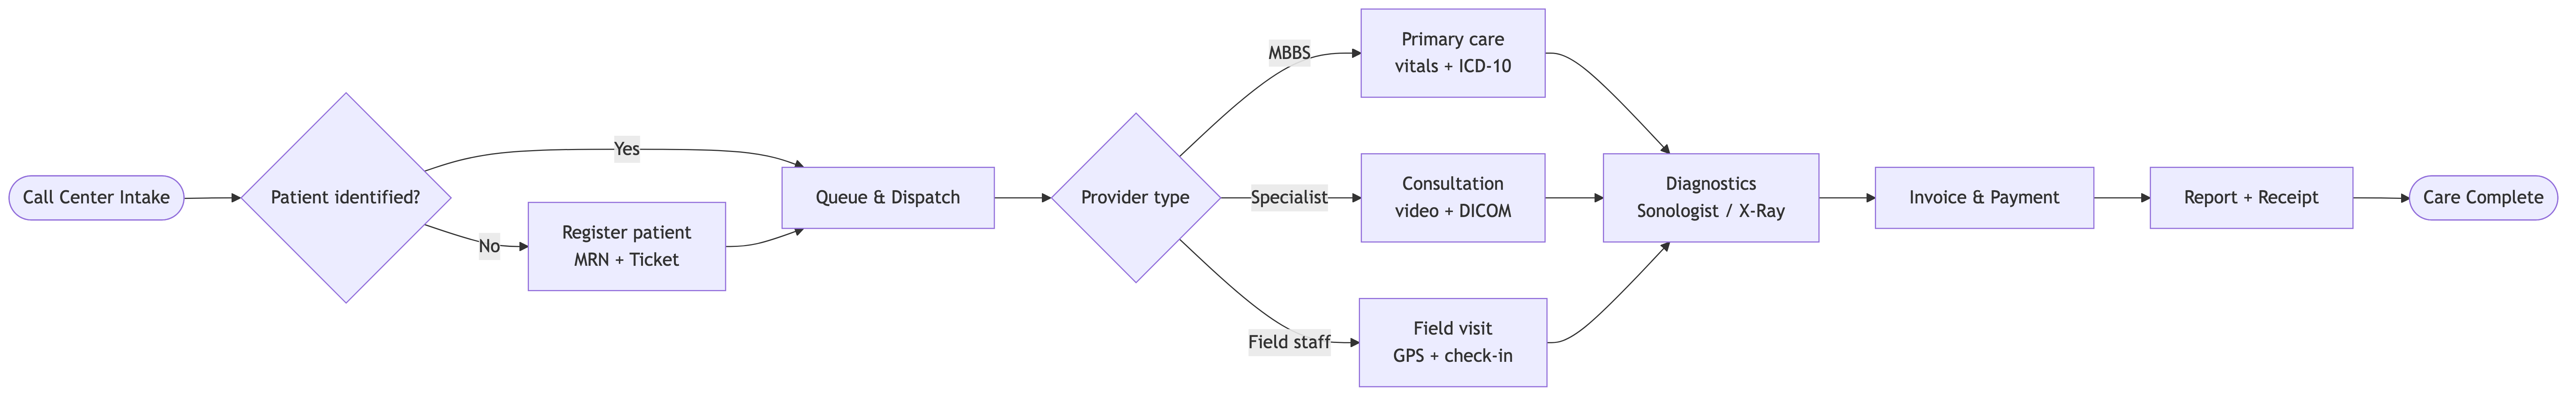
\includegraphics[width=\textwidth]{patient_flow_mermaid.png}
\caption{Patient journey through the HHDMS platform, from call-center intake and dispatch to consultation, diagnostics, and billing.}
\label{fig:patient_flow}
\end{figure*}

\section{Implementation Highlights}

The system was delivered through five weekly sprints targeting rapid SRS coverage~\cite{srs2026}. Key implementation decisions and techniques include:

\begin{itemize}
\item \textbf{Open-source field logistics:} The Google Maps dependency was replaced with an open-source mapping stack (osmdroid and the OSRM routing engine)~\cite{osmdroid2024}, enabling offline coordinate caching, geofenced check-ins, route deviation detection, and a live administrative tracking map without restrictive third-party quota limits.
\item \textbf{Unified notification engine:} External SMS and WhatsApp channels were deferred in favor of a reliable multi-channel engine built on Firebase Cloud Messaging push alerts~\cite{firebase2024fcm} with a backup polling loop, ensuring transactional delivery even in weak-signal environments.
\item \textbf{Standards-based imaging:} All diagnostic imaging was standardized on DICOM~\cite{dicom2021} and Cornerstone.js~, with an HTML5 Canvas annotation overlay shared across the specialist, sonologist, and X-ray workflows.
\item \textbf{Real-time WebSockets:} Socket.IO~\cite{fette2011websocket} was adopted for chat, video-call signaling, visit synchronization, and dashboard room updates, with compatibility flags for older Android clients.
\item \textbf{Transactional payments:} Stripe PaymentIntents and PaymentSheet~\cite{stripe2024api} were integrated end-to-end, with idempotent webhook handlers for automatic reconciliation.
\end{itemize}

The final system integrates more than ten roles across a secure, synchronized multi-tier ecosystem and reached staging deployment readiness.

\section{Development Methodology}

The project followed an agile, sprint-based methodology over five weekly iterations aligned with the course SRS~\cite{srs2026}. Each sprint began with a planning phase that decomposed pending SRS requirements into parallel development tracks, followed by implementation, integration, testing, and a weekly progress report. The team used a centralized version-controlled monorepo (Turborepo/npm workspaces for the backend and web, and a Gradle multi-module project for Android) to minimize integration conflicts across four parallel development streams.

A shared Prisma schema governed by a centralized PostgreSQL (Neon) database ensured that all modules operated against a consistent data model, with automated seeding scripts (guarded by a production host lock) populating multi-role mock records for staging. Each role-specific module was independently testable while remaining integrated through shared WebSocket, notification, and security primitives.

\section{Evaluation and Results}

The system was evaluated against the course Software Requirements Specification (SRS)~\cite{srs2026}, which defines the complete functional scope across all roles and subsystems.

\begin{itemize}
\item \textbf{SRS Coverage:} The delivered system achieved near-total coverage of the SRS. All primary clinical desks (MBBS, specialist, sonologist, X-ray), non-clinical desks (nutritionist, caregiver, nurse, call-center), and systemic engines (scheduling, billing, notifications, tracking, security) were operationalized.
\item \textbf{Integration:} The platform successfully unified disparate roles into a secure, synchronized multi-tier ecosystem, with cross-platform operations (web dashboards, mobile clients, and backend services) communicating without pipeline blockages~\cite{srs2026}.
\item \textbf{Staging Readiness:} The system was packaged as a runnable submission pre-populated with shared development credentials, enabling immediate execution against a pre-populated shared development database.
\item \textbf{Production-grade subsystems:} Critical functional domains---WebRTC video consultations~\cite{agorawebrtc}, interactive DICOM diagnostic tools~\cite{dicom2021}, real-time doctor--patient messaging~\cite{fette2011websocket}, Stripe payment gateways~\cite{stripe2024api}, and GPS-validated field operations~\cite{zandbergen2009accuracy}---were fully operationalized with persistent database support.
\end{itemize}

\section{Discussion}

The evaluation demonstrated that the HHDMS architecture meets its primary objective of consolidating fragmented home-healthcare workflows into a single, role-aware platform. Several design decisions materially influenced the outcome. First, the adoption of a unified Turborepo monorepo with a shared Prisma schema proved critical to integration quality: because all desks operate against one source of truth, cross-role state changes---such as a specialist referral flowing directly into the MBBS prescribing workspace---propagate without the manual reconciliation common to siloed healthcare product suites.

Second, real-time communication and diagnostics stood out as the highest-risk modules. The Socket.IO gateway---rather than a push-poll hybrid---was essential for acceptable teleconsultation latency, and its namespace isolation preserved security while keeping per-role state synchronized. Similarly, rendering diagnostics with the Cornerstone.js engine and a custom annotation overlay on device avoided the need to transmit heavyweight imaging workloads during consultations, keeping the expert-facing tools responsive even over constrained local-network links.

Third, the decision to defer proprietary Google Maps and SMS/WhatsApp channels in favor of the open-source OSRM/osmdroid stack and Firebase push notifications reflected a pragmatic scoping trade-off. It removed per-call external dependency risks and quota limits at the cost of offline-equatorial reach and richer messaging integrations.

Several limitations remain. The system was validated through staged mock data and coverage-based evaluation rather than a live clinical trial, so production-grade performance under real concurrency was not fully measured. Security hardening, while layered (JWT, RBAC, audit logging, PHI-conscious storage), has not been penetration-tested. Finally, the local-network server binding and source-hard-coded configuration constrain multi-site deployment and require operational attention before broad rollout. The platform currently offers no retrieval-augmented assistance for clinicians; introducing such capabilities would echo established retrieval-augmented generation techniques~\cite{rag2020} to surface relevant records and protocols. These considerations frame the future-work directions in the following section.

\section{Conclusion and Future Work}

HHDMS successfully demonstrates an integrated home healthcare management platform covering the complete patient lifecycle---from call-center intake and dispatch, through primary and specialist clinical care with telemedicine and DICOM diagnostics, to field logistics and automated billing. The system achieved near-total coverage of the course SRS and was packaged as a runnable submission with pre-populated shared development credentials.

Future work includes integrating a distributed message-queue topology (RabbitMQ/Redis) for resilient asynchronous messaging~\cite{catovic2022microservice}, expanding multi-method payment gateways (bKash, Nagad, Rocket), implementing an SMS/WhatsApp Business pipeline, and further hardening Protected Health Information (PHI) encryption and zero-trust RBAC compliance.

\bibliographystyle{IEEEtran}
\bibliography{ref}

\newpage
\onecolumn
\section*{Appendix}
\renewcommand{\thefigure}{\thesection-\arabic{figure}}
\addcontentsline{toc}{section}{Appendix}
\markboth{APPENDIX}{APPENDIX}

\section*{Appendix A: Modular Codebase Breakdown}

HHDMS was developed across two independent repositories: a Turborepo monorepo (the NestJS API and Next.js web application) and a Gradle multi-module Android project. Table~\ref{tab:modules} summarizes the primary modules and the file architecture of each.

\begin{table}[H]
\centering
\small
\renewcommand{\arraystretch}{1.2}
\begin{tabularx}{\textwidth}{>{\raggedright\arraybackslash}p{0.22\textwidth} >{\raggedright\arraybackslash}X >{\raggedright\arraybackslash}X}
\toprule
\textbf{Subsystem} & \textbf{Backend / Web Components} & \textbf{Android Components} \\
\midrule
Specialist & \texttt{specialist.service.ts}, \texttt{specialist-prescription.service.ts}, \texttt{drug-interactions.ts}, DICOM viewer (\texttt{dicom-viewer.tsx}, \texttt{dicom-canvas-overlay.tsx}) & \multicolumn{1}{c}{---} \\
Video Call & \texttt{video-call.gateway.ts}, \texttt{video-call.service.ts} & \texttt{VideoCallScreen.kt}, \texttt{IncomingVideoCallModal.kt}, \texttt{CallSignalingManager.kt} \\
MBBS & \texttt{mbbs.service.ts}, \texttt{mbbs.controller.ts}, \texttt{visit.gateway.ts} & \texttt{MbbsDoctorDashboardScreen.kt}, diagnosis/prescription/vitals/test/referral screens \\
Chat & \texttt{chat.service.ts}, \texttt{chat.gateway.ts}, \texttt{chat.controller.ts} & \texttt{ChatScreen.kt}, \texttt{ChatManager.kt} \\
Payments & \texttt{payments.service.ts}, \texttt{payments.controller.ts} & Stripe PaymentSheet in booking flow \\
Caregiver & \texttt{caregiver.service.ts}, \texttt{caregiver.controller.ts} & \texttt{CaregiverDashboardScreen.kt}, activity/condition/check-in screens \\
Sonologist & \texttt{sonologist.service.ts}, \texttt{sonologist.controller.ts} & \multicolumn{1}{c}{---} \\
Nutritionist & \texttt{nutritionist.service.ts}, \texttt{nutritionist.controller.ts}, \texttt{DietBuilder.tsx} & \multicolumn{1}{c}{---} \\
Nurse & nurse backend service & \texttt{:nurse} module (14 screens) \\
X-Ray & \texttt{xray\_*} Prisma models, technician/exposure UI & \multicolumn{1}{c}{---} \\
\bottomrule
\end{tabularx}
\caption{HHDMS module breakdown by subsystem.}
\label{tab:modules}
\end{table}

\section*{Appendix B: Technology Stack}

Table~\ref{tab:stack} enumerates the technologies used across the stack.

\begin{table}[H]
\centering
\small
\renewcommand{\arraystretch}{1.2}
\begin{tabularx}{\textwidth}{>{\raggedright\arraybackslash}p{0.20\textwidth} >{\raggedright\arraybackslash}X}
\toprule
\textbf{Layer} & \textbf{Technologies} \\
\midrule
Backend & NestJS 11, Prisma ORM, PostgreSQL (Neon), Passport JWT, Socket.IO, Firebase Admin SDK, Stripe SDK, Agora Token Builder \\
Web & Next.js 16 (App Router), Tailwind CSS v4, Socket.IO client, Cornerstone.js (DICOM), html2canvas/jsPDF (PDF export) \\
Android & Jetpack Compose, Material 3, Retrofit 2.11, Socket.IO 2.1.1, Agora RTC SDK 4.6.3, osmdroid 6.1.18, Stripe Android 20.48.1, Firebase Messaging KTX, Play Services Location \\
Infrastructure & Turborepo monorepo (npm workspaces), Gradle multi-module Android \\
\bottomrule
\end{tabularx}
\caption{Technology stack of HHDMS.}
\label{tab:stack}
\end{table}

\section*{Appendix C: SRS Coverage Mapping}

The delivered system was mapped against the major functional requirement groups of the course SRS~\cite{srs2026}. Table~\ref{tab:srs} records the coverage status and the implementing subsystem for each group.

\begin{table}[H]
\centering
\small
\renewcommand{\arraystretch}{1.2}
\begin{tabularx}{\textwidth}{>{\raggedright\arraybackslash}p{0.30\textwidth} >{\raggedright\arraybackslash}X >{\raggedright\arraybackslash}p{0.14\textwidth}}
\toprule
\textbf{SRS Requirement Group} & \textbf{Implementing Subsystem} & \textbf{Status} \\
\midrule
Call-center intake and dispatch & Call-Center Dispatch, ticketing, emergency triage & Complete \\
Primary-care consultation & MBBS module (vitals, ICD-10, prescriptions, referrals) & Complete \\
Specialist consultation & Specialist module, dynamic templates, drug interactions & Complete \\
Medical imaging & Sonologist, X-Ray, DICOM viewer suite & Complete \\
Telehealth & Video consultation, chat, notifications & Complete \\
Field operations & Caregiver module, GPS telemetry, geofencing & Complete \\
Nutrition & Nutritionist workbench, diet planner, adherence & Complete \\
Nursing & Standalone nurse Android app + backend & Complete \\
Billing \& payments & Invoice engine, Stripe PaymentIntents & Complete \\
Administration & Admin dashboard, analytics, scheduling & Complete \\
Security & JWT auth, RBAC, audit logging & Complete \\
\bottomrule
\end{tabularx}
\caption{SRS requirement-group coverage.}
\label{tab:srs}
\end{table}

\section*{Appendix D: Major API Endpoint Families}

Table~\ref{tab:api} lists the primary REST and WebSocket endpoint families exposed by the backend.

\begin{table}[H]
\centering
\small
\renewcommand{\arraystretch}{1.2}
\begin{tabularx}{\textwidth}{>{\raggedright\arraybackslash}p{0.22\textwidth} >{\raggedright\arraybackslash}X >{\raggedright\arraybackslash}X}
\toprule
\textbf{Module} & \textbf{REST Endpoint Family} & \textbf{WebSocket Events} \\
\midrule
MBBS & \texttt{/mbbs/vitals}, \texttt{/mbbs/diagnoses}, \texttt{/mbbs/prescriptions}, \texttt{/mbbs/referrals}, \texttt{/mbbs/test-orders}, \texttt{/mbbs/emergency}, \texttt{/mbbs/signature} & \texttt{visit:*}, \texttt{appointment:update} \\
Specialist & \texttt{/specialist/referrals}, \texttt{/specialist/prescriptions}, \texttt{/specialist/reports}, \texttt{/specialist/templates}, \texttt{/specialist/dicom} & \multicolumn{1}{c}{---} \\
Chat & \texttt{/chat/conversations}, \texttt{/chat/messages} & \texttt{chat:join}, \texttt{chat:message}, \texttt{chat:typing} \\
Payments & \texttt{/payments/intent}, \texttt{/payments/confirm}, \texttt{/payments/webhook} & \multicolumn{1}{c}{---} \\
Caregiver & \texttt{/caregiver/profiles}, \texttt{/caregiver/activities}, \texttt{/caregiver/reports}, \texttt{/caregiver/check-in}, \texttt{/caregiver/timesheets} & \multicolumn{1}{c}{---} \\
Nutritionist & \texttt{/nutritionist/anthropometric}, \texttt{/nutritionist/diet-plans}, \texttt{/nutritionist/meals}, \texttt{/nutritionist/adherence}, \texttt{/nutritionist/follow-ups}, \texttt{/nutritionist/nutrients} & \multicolumn{1}{c}{---} \\
Sonologist & \texttt{/sonologist/studies}, \texttt{/sonologist/reports} & \multicolumn{1}{c}{---} \\
Tracking & \texttt{/tracking/location} & \texttt{tracking:stream} \\
\bottomrule
\end{tabularx}
\caption{Major endpoint families by module.}
\label{tab:api}
\end{table}


\end{document}
